% This LaTeX document needs to be compiled with XeLaTeX.
\documentclass[10pt]{article}
\usepackage[utf8]{inputenc}
\usepackage{ucharclasses}
\usepackage{graphicx}
\usepackage[export]{adjustbox}
\graphicspath{ {./images/} }
\usepackage{amsmath}
\usepackage{amsfonts}
\usepackage{amssymb}
\usepackage[version=4]{mhchem}
\usepackage{stmaryrd}
\usepackage{hyperref}
\hypersetup{colorlinks=true, linkcolor=blue, filecolor=magenta, urlcolor=cyan,}
\urlstyle{same}
\usepackage{multirow}
\usepackage[fallback]{xeCJK}
\usepackage{polyglossia}
\usepackage{fontspec}
\setCJKmainfont{Noto Serif CJK KR}

\setmainlanguage{polish}
\setotherlanguages{hindi, bengali}
\newfontfamily\hindifont{Noto Serif Devanagari}
\newfontfamily\bengalifont{Noto Serif Bengali}
\newfontfamily\lgcfont{CMU Serif}
\setDefaultTransitions{\lgcfont}{}
\setTransitionsFor{Hindi}{\hindifont}{\lgcfont}
\setTransitionsFor{Bengali}{\bengalifont}{\lgcfont}

\title{KOD }

\author{}
\date{}


\newcommand\Varangle{\mathop{{<\!\!\!\!\!\text{\small)}}\:}\nolimits}

\begin{document}
\maketitle
IMIĘ I NAZWISKO *\\
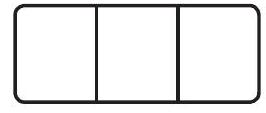
\includegraphics[max width=\textwidth, center]{2024_11_21_72158d4a4efa7dd894bcg-01}\\
\(\square\)

\begin{itemize}
  \item nieobowiązkowe
\end{itemize}

\section*{PRÓBNY EGZAMIN MATURALNY Z NOWĄ ERĄ MATEMATYKA - POZIOM PODSTAWOWY}
\section*{Instrukcja dla zdającego}
\begin{enumerate}
  \item Sprawdź, czy arkusz egzaminacyjny zawiera 24 strony (zadania 1-33) i kartę odpowiedzi. Ewentualny brak stron zgłoś nauczycielowi nadzorującemu egzamin.
  \item Rozwiązania zadań i odpowiedzi zapisz w miejscu na to przeznaczonym.
  \item Pamiętaj, że pominięcie argumentacji lub istotnych obliczeń w rozwiązaniu zadań otwartych może spowodować, że za to rozwiązanie nie otrzymasz pełnej liczby punktów.
  \item Pisz czytelnie. Używaj długopisu/pióra tylko z czarnym tuszem/atramentem.
  \item Nie używaj korektora, a błędne zapisy wyraźnie przekreśl.
  \item Pamiętaj, że zapisy w brudnopisie nie będą oceniane.
  \item Podczas egzaminu możesz korzystać z zestawu wzorów matematycznych, cyrkla i linijki oraz kalkulatora prostego.
  \item Na tej stronie i na karcie odpowiedzi wpisz swój kod oraz imię i nazwisko.
  \item Odpowiedzi do zadań zamkniętych przenieś na kartę odpowiedzi, zaznaczając je w części karty przeznaczonej dla zdającego.
  \item Nie wpisuj żadnych znaków w części przeznaczonej dla osoby sprawdzającej.\\
\(\square\) dysleksja
\end{enumerate}

STYCZEŃ 2016

Czas pracy:\\
170 minut

Liczba punktów\\
do uzyskania: 50

W zadaniach od 1. do 23. wybierz i zaznacz na karcie odpowiedzi poprawna odpowiedź.

\section*{Zadanie 1. (0-1)}
Liczba 60 jest przybliżeniem z niedomiarem liczby \(x\). Błąd względny tego przybliżenia to \(4 \%\). Liczba \(x\) jest równa\\
A. 57,69\\
B. 57,6\\
C. 60,04\\
D. 62,5

\section*{Zadanie 2. (0-1)}
Dla liczb \(a=2 \sqrt{2} \mathrm{i} b=\sqrt{2-\sqrt{2}}\) wyrażenie \(\frac{a}{b^{2}}\) jest równe\\
A. \(2 \sqrt{2}-2\)\\
B. 2\\
C. \(2(\sqrt{2}+1)\)\\
D. \(4(2+\sqrt{2})\)

\section*{Zadanie 3. (0-1)}
Cenę towaru podwyższono o \(20 \%\). O ile procent należy obniżyć nową cenę towaru, aby po obniżce stanowiła ona \(90 \%\) ceny przed zmianami?\\
A. o 10\%\\
B. o \(15 \%\)\\
C. o 25\%\\
D. o \(30 \%\)

\section*{Zadanie 4. (0-1)}
Ciąg \(\left(a_{n}\right)\) jest określony wzorem \(a_{n}=\log (n+1)\) dla \(n \geqslant 1\). Liczba \(\frac{3 a_{3}-a_{7}}{a_{1}}\) jest równa\\
A. \(\log 4\)\\
B. \(\log 6\)\\
C. 2\\
D. 3

Zadanie 5. (0-1)\\
Iloraz liczby \(8^{10}-4^{14}\) przez liczbę \(6 \sqrt[3]{4} \cdot \sqrt[6]{4}\) jest równy\\
A. \(\frac{1}{3}\)\\
B. \(\frac{1}{6}\)\\
C. \(2^{26}\)\\
D. \(2^{30}\)

\section*{Zadanie 6. (0-1)}
Równanie \(\frac{8-2 x^{2}}{x+2}=x+2\) ma dokładnie\\
A. dwa rozwiązania: \(x_{1}=\frac{2}{\sqrt{3}}, x_{2}=-\frac{2}{\sqrt{3}}\).\\
B. dwa rozwiązania: \(x=\frac{2}{3}, x=-2\).\\
C. jedno rozwiązanie: \(x=2\).\\
D. jedno rozwiązanie: \(x=\frac{2}{3}\).

Więcej arkuszy znajdziesz na stronie: \href{http://arkusze.pl}{arkusze.pl}\\

\includegraphics[max width=\textwidth, center]{2024_11_21_72158d4a4efa7dd894bcg-03}

Zadanie 7. (0-1)\\
Liczba 4 spełnia nierówność \(a^{2} x-16<0 \mathrm{z}\) niewiadomą \(x\) wtedy i tylko wtedy, gdy\\
A. \(a \in(-2,2)\)\\
B. \(a \in(-\infty,-2) \cup(2, \infty)\)\\
C. \(a \in\{-2,2\}\)\\
D. \(a \in(-\infty, 2)\)

\section*{Zadanie 8. (0-1)}
Funkcja \(f\) przyporządkowuje każdej liczbie naturalnej \(n\) największy wspólny dzielnik liczb \(n\) oraz \(n+10\). Największa wartość funkcji \(f\) jest równa\\
A. 2\\
B. 5\\
C. 10\\
D. 20

\section*{Zadanie 9. (0-1)}
Funkcja liniowa \(f(x)=-2 x+b\) przyjmuje wartości dodatnie dla wszystkich \(x<2\) i tylko dla takich. Wynika stąd, że współczynnik \(b\) jest równy\\
A. 4\\
B. 2\\
C. 0\\
D. -4

Zadanie 10. (0-1)\\
Prostą o równaniu \(y=\frac{1}{2} x+1\) przesunięto wzdłuż osi \(O x\) o cztery jednostki w prawo. Otrzymano prostą o równaniu\\
A. \(y=\frac{1}{2} x-3\)\\
B. \(y=\frac{1}{2} x-1\)\\
C. \(y=\frac{1}{2} x+3\)\\
D. \(y=\frac{1}{2} x+5\)

\section*{Zadanie 11. (0-1)}
Wykres funkcji kwadratowej \(f(x)=-(x+1)^{2}+5\) przekształcono symetrycznie względem osi \(O y\) i otrzymano wykres funkcji \(g\). Wskaż równanie prostej, która jest osią symetrii wykresu funkcji \(g\).\\
A. \(x=1\)\\
B. \(x=-1\)\\
C. \(y=5\)\\
D. \(y=1\)

\section*{Zadanie 12. (0-1)}
Pan Krzysztof pokonuje trasę Warszawa-Kraków w czasie \(t\) ze średnią prędkością v. Aby skrócić czas podróży o 20\%, pan Krzysztof musi średnią prędkość\\
A. zwiększyć o 25\%.\\
B. zwiększyć o 20\%.\\
C. zmniejszyć o 20\%.\\
D. zmniejszyć o 25\%.

Więcej arkuszy znajdziesz na stronie: \href{http://arkusze.pl}{arkusze.pl}\\

\includegraphics[max width=\textwidth, center]{2024_11_21_72158d4a4efa7dd894bcg-05}

\section*{Zadanie 13. (0-1)}
Ciąg \(\left(a_{n}\right)\) jest określony wzorem \(a_{n}=\frac{3}{4} n^{2}-24 n+90\) dla \(n \geqslant 1\). Najmniejszy wyraz ciągu \(\left(a_{n}\right)\) jest równy\\
A. 90\\
B. \(66 \frac{3}{4}\)\\
C. -102\\
D. -124

\section*{Zadanie 14. (0-1)}
Dla pewnego kąta ostrego \(\alpha\) trzywyrazowy ciąg \(\left(2 \sin ^{2} \alpha, \sqrt{3} \operatorname{tg} \alpha, 2 \cos ^{2} \alpha\right)\) jest arytmetyczny. Miara kąta \(\alpha\) jest równa\\
A. \(75^{\circ}\)\\
B. \(60^{\circ}\)\\
C. \(45^{\circ}\)\\
D. \(30^{\circ}\)

\section*{Zadanie 15. (0-1)}
Kąt \(\alpha\) jest kątem ostrym w trójkącie prostokątnym przedstawionym na rysunku.\\
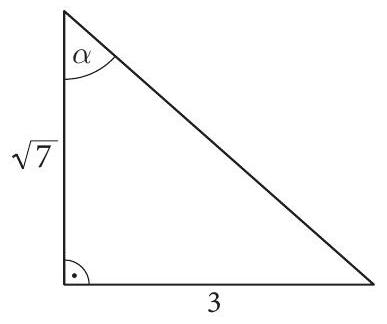
\includegraphics[max width=\textwidth, center]{2024_11_21_72158d4a4efa7dd894bcg-06}

Liczba \(4^{\text {sin } \alpha}\) jest równa\\
A. \(\sqrt{2^{\sqrt{7}}}\)\\
B. \(2 \sqrt{2}\)\\
C. \(4^{\frac{3}{7}}\)\\
D. \(4 \sqrt[3]{4}\)

\section*{Zadanie 16. (0-1)}
Prosta o równaniu \(y=-2 x\) tworzy z osią \(O x\) kąt rozwarty \(\alpha\) (zobacz rysunek poniżej).\\
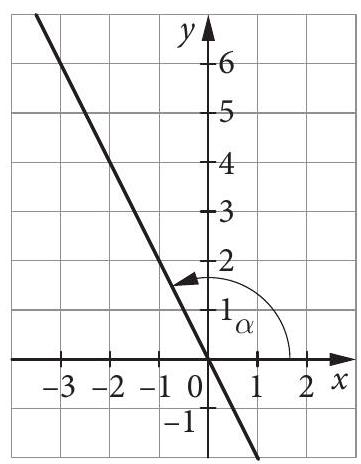
\includegraphics[max width=\textwidth, center]{2024_11_21_72158d4a4efa7dd894bcg-06(1)}

Cosinus kąta \(\alpha\) jest równy\\
A. -2\\
B. \(-\frac{1}{2}\)\\
C. \(\frac{2 \sqrt{5}}{5}\)\\
D. \(-\frac{\sqrt{5}}{5}\)

Więcej arkuszy znajdziesz na stronie: \href{http://arkusze.pl}{arkusze.pl}\\

\includegraphics[max width=\textwidth, center]{2024_11_21_72158d4a4efa7dd894bcg-07}

\section*{Zadanie 17. (0-1)}
W okrąg o środku \(S\) wpisano deltoid \(A B C D\) (zobacz rysunek poniżej). Krótsza przekątna deltoidu ma długość 4 , a jego najmniejszy kąt wewnętrzny ma miarę \(45^{\circ}\).\\
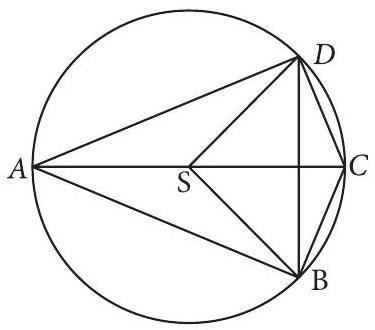
\includegraphics[max width=\textwidth, center]{2024_11_21_72158d4a4efa7dd894bcg-08}

Pole deltoidu jest równe\\
A. \(16 \sqrt{2}\)\\
B. 16\\
C. 12\\
D. \(8 \sqrt{2}\)

\section*{Zadanie 18. (0-1)}
Dwa okręgi: pierwszy o środku \(O_{1}=(-2,4)\) i promieniu \(r_{1}=4\) oraz drugi o środku \(O_{2}=(6,0)\), są styczne zewnętrznie. Promień drugiego okręgu jest równy\\
A. 4\\
B. \(4(\sqrt{5}-1)\)\\
C. \(2 \sqrt{5}\)\\
D. 5

\section*{Zadanie 19. (0-1)}
Rysunek przedstawia ostrosłup prawidłowy trójkątny.\\
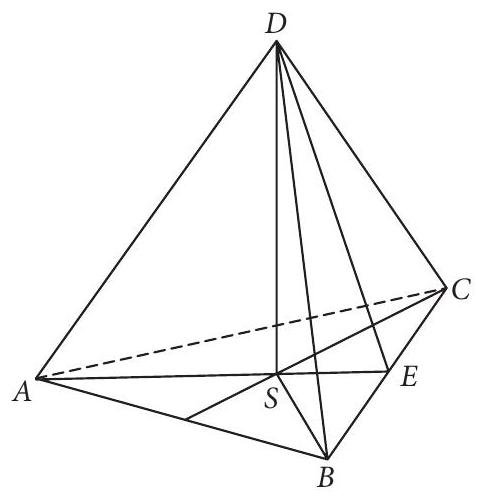
\includegraphics[max width=\textwidth, center]{2024_11_21_72158d4a4efa7dd894bcg-08(1)}

Kąt między ścianą boczną a płaszczyzną podstawy ostrosłupa to\\
A. \(\Varangle D E S\)\\
B. \(\Varangle D C E\)\\
C. \(\Varangle D C S\)\\
D. \(\Varangle D E B\)

\section*{Zadanie 20. (0-1)}
Pole powierzchni bocznej walca jest 5 razy większe od sumy pól jego podstaw. Miara kąta nachylenia przekątnej przekroju osiowego tego walca do podstawy jest w przybliżeniu równa\\
A. \(79^{\circ}\)\\
B. \(68^{\circ}\)\\
C. \(51^{\circ}\)\\
D. \(22^{\circ}\)

Więcej arkuszy znajdziesz na stronie: \href{http://arkusze.pl}{arkusze.pl}\\

\includegraphics[max width=\textwidth, center]{2024_11_21_72158d4a4efa7dd894bcg-09}

\section*{Zadanie 21. (0-1)}
Laura ma pięć płyt z muzyką taneczną i trzy z muzyką poważną. Na ile sposobów Laura może tak ustawić poszczególne płyty na półce, aby wszystkie płyty tego samego gatunku znalazły się obok siebie? Wskaż poprawny sposób obliczeń.\\
A. \(5 \cdot 4 \cdot 3 \cdot 2 \cdot 1 \cdot 3 \cdot 2 \cdot 1\)\\
B. \(5 \cdot 4 \cdot 3 \cdot 2 \cdot 1+3 \cdot 2 \cdot 1\)\\
C. \(2 \cdot 5 \cdot 4 \cdot 3 \cdot 2 \cdot 1 \cdot 3 \cdot 2 \cdot 1\)\\
D. \(2 \cdot 5^{5} \cdot 3^{3}\)

\section*{Zadanie 22. (0-1)}
W tabeli podano oceny z matematyki czterech uczniów pewnej klasy.

\begin{center}
\begin{tabular}{|c|c|}
\hline
Uczeń & Oceny \\
\hline
Ada & \(4,4,4,5,5\) \\
\hline
Basia & \(3,3,3,4,4\) \\
\hline
Czarek & \(1,1,2,2,2\) \\
\hline
Darek & \(1,1,5,5,5\) \\
\hline
\end{tabular}
\end{center}

Oceny którego ucznia wykazują największe odchylenie standardowe?\\
A. Ady\\
B. Basi\\
C. Czarka\\
D. Darka

\section*{Zadanie 23. (0-1)}
W urnie jest o 10 kul białych więcej niż czarnych. Z urny losujemy jedną kulę. Prawdopodobieństwo wylosowania kuli białej jest równe \(\frac{3}{4}\). Ile wszystkich kul jest w urnie?\\
A. 15\\
B. 20\\
C. 30\\
D. 40

Więcej arkuszy znajdziesz na stronie: \href{http://arkusze.pl}{arkusze.pl}\\

\includegraphics[max width=\textwidth, center]{2024_11_21_72158d4a4efa7dd894bcg-11}

Zadanie 24. (0-2)\\
Wyznacz zbiór wszystkich argumentów \(x\), dla których funkcja kwadratowa \(f(x)=\frac{1}{2} x^{2}+2 x+2\) przyjmuje większe wartości niż funkcja liniowa \(g(x)=-x+2\).

Więcej arkuszy znajdziesz na stronie: \href{http://arkusze.pl}{arkusze.pl}\\

\includegraphics[max width=\textwidth, center]{2024_11_21_72158d4a4efa7dd894bcg-12}

Odpowiedź:

\section*{Zadanie 25. (0-2)}
Dla jakich wartości \(m\) równanie \(x(3 x-6)\left(x^{3}+27\right)(x+m)=0 \mathrm{z}\) niewiadomą \(x\) ma trzy różne rozwiązania?

Więcej arkuszy znajdziesz na stronie: \href{http://arkusze.pl}{arkusze.pl}

\begin{center}
\begin{tabular}{|c|c|c|c|c|c|c|c|c|c|c|c|c|c|c|c|c|c|c|c|c|c|c|c|c|c|c|c|c|c|}
\hline
 &  &  &  &  &  &  &  &  &  &  &  &  &  &  &  &  &  &  &  &  &  &  &  &  &  &  &  &  &  \\
\hline
 &  &  &  &  &  &  &  &  &  &  &  &  &  &  &  &  &  &  &  &  &  &  &  &  &  &  &  &  &  \\
\hline
 &  &  &  &  &  &  &  &  &  &  &  &  &  &  &  &  &  &  &  &  &  &  &  &  &  &  &  &  &  \\
\hline
 &  &  &  &  &  &  &  &  &  &  &  &  &  &  &  &  &  &  &  &  &  &  &  &  &  &  &  &  &  \\
\hline
 &  &  &  &  &  &  &  &  &  &  &  &  &  &  &  &  &  &  &  &  &  &  &  &  &  &  &  &  &  \\
\hline
 &  &  &  &  &  &  &  &  &  &  &  &  &  &  &  &  &  &  &  &  &  &  &  &  &  &  &  &  &  \\
\hline
 &  &  &  &  &  &  &  &  &  &  &  &  &  &  &  &  &  &  &  &  &  &  &  &  &  &  &  &  &  \\
\hline
 &  &  &  &  &  &  &  &  &  &  &  &  &  &  &  &  &  &  &  &  &  &  &  &  &  &  &  &  &  \\
\hline
 &  &  &  &  &  &  &  &  &  &  &  &  &  &  &  &  &  &  &  &  &  &  &  &  &  &  &  &  &  \\
\hline
 &  &  &  &  &  &  &  &  &  &  &  &  &  &  &  &  &  &  &  &  &  &  &  &  &  &  &  &  &  \\
\hline
 &  &  &  &  &  &  &  &  &  &  &  &  &  &  &  &  &  &  &  &  &  &  &  &  &  &  &  &  &  \\
\hline
 &  &  &  &  &  &  &  &  &  &  &  &  &  &  &  &  &  &  &  &  &  &  &  &  &  &  &  &  &  \\
\hline
 &  &  &  &  &  &  &  &  &  &  &  &  &  &  &  &  &  &  &  &  &  &  &  &  &  &  &  &  &  \\
\hline
 &  &  &  &  &  &  &  &  &  &  &  &  &  &  &  &  &  &  &  &  &  &  &  &  &  &  &  &  &  \\
\hline
 &  &  &  &  &  &  &  &  &  &  &  &  &  &  &  &  &  &  &  &  &  &  &  &  &  &  &  &  &  \\
\hline
 &  &  &  &  &  &  &  &  &  &  &  &  &  &  &  &  &  &  &  &  &  &  &  &  &  &  &  &  &  \\
\hline
 &  &  &  &  &  &  &  &  &  &  &  &  &  &  &  &  &  &  &  &  &  &  &  &  &  &  &  &  &  \\
\hline
 &  &  &  &  &  &  &  &  &  &  &  &  &  &  &  &  &  &  &  &  &  &  &  &  &  &  &  &  &  \\
\hline
 &  &  &  &  &  &  &  &  &  &  &  &  &  &  &  &  &  &  &  &  &  &  &  &  &  &  &  &  &  \\
\hline
 &  &  &  &  &  &  &  &  &  &  &  &  &  &  &  &  &  &  &  &  &  &  &  &  &  &  &  &  &  \\
\hline
 &  &  &  &  &  &  &  &  &  &  &  &  &  &  &  &  &  &  &  &  &  &  &  &  &  &  &  &  &  \\
\hline
 &  &  &  &  &  &  &  &  &  &  &  &  &  &  &  &  &  &  &  &  &  &  &  &  &  &  &  &  &  \\
\hline
 &  &  &  &  &  &  &  &  &  &  &  &  &  &  &  &  &  &  &  &  &  &  &  &  &  &  &  &  &  \\
\hline
 &  &  &  &  &  &  &  &  &  &  &  &  &  &  &  &  &  &  &  &  &  &  &  &  &  &  &  &  &  \\
\hline
 &  &  &  &  &  &  &  &  &  &  &  &  &  &  &  &  &  &  &  &  &  &  &  &  &  &  &  &  &  \\
\hline
 &  &  &  &  &  &  &  &  &  &  &  &  &  &  &  &  &  &  &  &  &  &  &  &  &  &  &  &  &  \\
\hline
 &  &  &  &  &  &  &  &  &  &  &  &  &  &  &  &  &  &  &  &  &  &  &  &  &  &  &  &  &  \\
\hline
 &  &  &  &  &  &  &  &  &  &  &  &  &  &  &  &  &  &  &  &  &  &  &  &  &  &  &  &  &  \\
\hline
 &  &  &  &  &  &  &  &  &  &  &  &  &  &  &  &  &  &  &  &  &  &  &  &  &  &  &  &  &  \\
\hline
 &  &  &  &  &  &  &  &  &  &  &  &  &  &  &  &  &  &  &  &  &  &  &  &  &  &  &  &  &  \\
\hline
 &  &  &  &  &  &  &  &  &  &  &  &  &  &  &  &  &  &  &  &  &  &  &  &  &  &  &  &  &  \\
\hline
 &  &  &  &  &  &  &  &  &  &  &  &  &  &  &  &  &  &  &  &  &  &  &  &  &  &  &  &  &  \\
\hline
 &  &  &  &  &  &  &  &  &  &  &  &  &  &  &  &  &  &  &  &  &  &  &  &  &  &  &  &  &  \\
\hline
 &  &  &  &  &  &  &  &  &  &  &  &  &  &  &  &  &  &  &  &  &  &  &  &  &  &  &  &  &  \\
\hline
 &  &  &  &  &  &  &  &  &  &  &  &  &  &  &  &  &  &  &  &  &  &  &  &  &  &  &  &  &  \\
\hline
 &  &  &  &  &  &  &  &  &  &  &  &  &  &  &  &  &  &  &  &  &  &  &  &  &  &  &  &  &  \\
\hline
 &  &  &  &  &  &  &  &  &  &  &  &  &  &  &  &  &  &  &  &  &  &  &  &  &  &  &  &  &  \\
\hline
\end{tabular}
\end{center}

Odpowiedź:

\begin{center}
\begin{tabular}{|l|l|c|c|}
\hline
\multirow{2}{*}{\begin{tabular}{c}
Wypełnia \\
sprawdzający \\
\end{tabular}} & Nr zadania & 24 & 25 \\
\cline { 2 - 4 }
 & Maks. liczba pkt & 2 & 2 \\
\cline { 2 - 4 }
 & Uzyskana liczba pkt &  &  \\
\hline
\end{tabular}
\end{center}

Zadanie 26. (0-2)\\
Ustalono, że w pewnym jeziorze populacja zagrożonego gatunku ryb maleje każdego roku o 30\%, a na początku badań wynosiła 50 tys. sztuk. Podaj wzór funkcji wyrażającej liczebność tej populacji po upływie \(t\) lat i oblicz, ile ryb zagrożonego gatunku było w jeziorze po trzech latach od chwili rozpoczęcia badań.

Więcej arkuszy znajdziesz na stronie: \href{http://arkusze.pl}{arkusze.pl}\\

\includegraphics[max width=\textwidth, center]{2024_11_21_72158d4a4efa7dd894bcg-14}

Odpowiedź:

Zadanie 27. (0-2)\\
Udowodnij, że różnica kwadratów dowolnej liczby pierwszej \(p>2\) i liczby o dwa od niej mniejszej jest podzielna przez 8.

Więcej arkuszy znajdziesz na stronie: \href{http://arkusze.pl}{arkusze.pl}\\

\includegraphics[max width=\textwidth, center]{2024_11_21_72158d4a4efa7dd894bcg-15}

\begin{center}
\begin{tabular}{|l|l|c|c|}
\hline
\multirow{2}{*}{\begin{tabular}{c}
Wypełnia \\
sprawdzający \\
\end{tabular}} & Nr zadania & 26 & 27 \\
\cline { 2 - 4 }
 & Maks. liczba pkt & 2 & 2 \\
\cline { 2 - 4 }
 & Uzyskana liczba pkt &  &  \\
\hline
\end{tabular}
\end{center}

\section*{Zadanie 28. (0-2)}
W trapezie prostokątnym \(A B C D\), w którym \(A B \| C D\) i \(|A B|=2|C D|\), poprowadzono przekątne \(A C\) i \(B D\), przecinające się w punkcie \(S\). Udowodnij, że odległość punktu \(S\) od ramienia \(A D\), prostopadłego do podstaw, jest trzy razy mniejsza niż długość podstawy \(A B\).\\
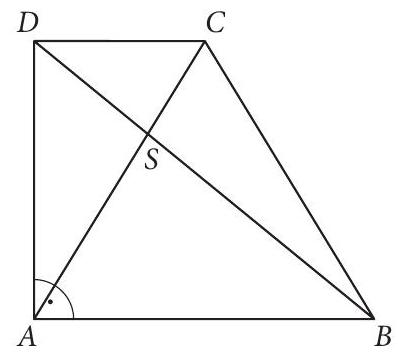
\includegraphics[max width=\textwidth, center]{2024_11_21_72158d4a4efa7dd894bcg-16}\\

\includegraphics[max width=\textwidth, center]{2024_11_21_72158d4a4efa7dd894bcg-16(1)}

Zadanie 29. (0-2)\\
Punkty \(A=(-2 \sqrt{3}, 0), B=(0,0), C=(\sqrt{3}, 3)\) są kolejnymi wierzchołkami sześciokąta foremnego \(A B C D E F\). Wyznacz równanie prostej zawierającej przekątną \(A D\) tego sześciokąta.\\
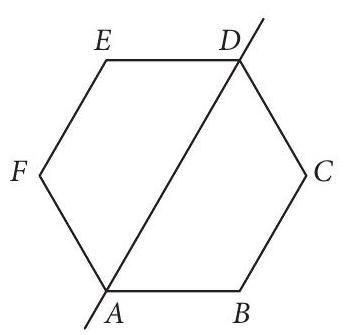
\includegraphics[max width=\textwidth, center]{2024_11_21_72158d4a4efa7dd894bcg-17}

Więcej arkuszy znajdziesz na stronie: \href{http://arkusze.pl}{arkusze.pl}

\begin{center}
\begin{tabular}{|c|c|c|c|c|c|c|c|c|c|c|c|c|c|c|c|c|c|c|c|c|c|c|c|c|c|c|c|c|c|}
\hline
 &  &  &  &  &  &  &  &  &  &  &  &  &  &  &  &  &  &  &  &  &  &  &  &  &  &  &  &  &  \\
\hline
 &  &  &  &  &  &  &  &  &  &  &  &  &  &  &  &  &  &  &  &  &  &  &  &  &  &  &  &  &  \\
\hline
 &  &  &  &  &  &  &  &  &  &  &  &  &  &  &  &  &  &  &  &  &  &  &  &  &  &  &  &  &  \\
\hline
 &  &  &  &  &  &  &  &  &  &  &  &  &  &  &  &  &  &  &  &  &  &  &  &  &  &  &  &  &  \\
\hline
 &  &  &  &  &  &  &  &  &  &  &  &  &  &  &  &  &  &  &  &  &  &  &  &  &  &  &  &  &  \\
\hline
 &  &  &  &  &  &  &  &  &  &  &  &  &  &  &  &  &  &  &  &  &  &  &  &  &  &  &  &  &  \\
\hline
 &  &  &  &  &  &  &  &  &  &  &  &  &  &  &  &  &  &  &  &  &  &  &  &  &  &  &  &  &  \\
\hline
 &  &  &  &  &  &  &  &  &  &  &  &  &  &  &  &  &  &  &  &  &  &  &  &  &  &  &  &  &  \\
\hline
 &  &  &  &  &  &  &  &  &  &  &  &  &  &  &  &  &  &  &  &  &  &  &  &  &  &  &  &  &  \\
\hline
 &  &  &  &  &  &  &  &  &  &  &  &  &  &  &  &  &  &  &  &  &  &  &  &  &  &  &  &  &  \\
\hline
 &  &  &  &  &  &  &  &  &  &  &  &  &  &  &  &  &  &  &  &  &  &  &  &  &  &  &  &  &  \\
\hline
 &  &  &  &  &  &  &  &  &  &  &  &  &  &  &  &  &  &  &  &  &  &  &  &  &  &  &  &  &  \\
\hline
 &  &  &  &  &  &  &  &  &  &  &  &  &  &  &  &  &  &  &  &  &  &  &  &  &  &  &  &  &  \\
\hline
 &  &  &  &  &  &  &  &  &  &  &  &  &  &  &  &  &  &  &  &  &  &  &  &  &  &  &  &  &  \\
\hline
 &  &  &  &  &  &  &  &  &  &  &  &  &  &  &  &  &  &  &  &  &  &  &  &  &  &  &  &  &  \\
\hline
 &  &  &  &  &  &  &  &  &  &  &  &  &  &  &  &  &  &  &  &  &  &  &  &  &  &  &  &  &  \\
\hline
 &  &  &  &  &  &  &  &  &  &  &  &  &  &  &  &  &  &  &  &  &  &  &  &  &  &  &  &  &  \\
\hline
 &  &  &  &  &  &  &  &  &  &  &  &  &  &  &  &  &  &  &  &  &  &  &  &  &  &  &  &  &  \\
\hline
 &  &  &  &  &  &  &  &  &  &  &  &  &  &  &  &  &  &  &  &  &  &  &  &  &  &  &  &  &  \\
\hline
 &  &  &  &  &  &  &  &  &  &  &  &  &  &  &  &  &  &  &  &  &  &  &  &  &  &  &  &  &  \\
\hline
 &  &  &  &  &  &  &  &  &  &  &  &  &  &  &  &  &  &  &  &  &  &  &  &  &  &  &  &  &  \\
\hline
 &  &  &  &  &  &  &  &  &  &  &  &  &  &  &  &  &  &  &  &  &  &  &  &  &  &  &  &  &  \\
\hline
 &  &  &  &  &  &  &  &  &  &  &  &  &  &  &  &  &  &  &  &  &  &  &  &  &  &  &  &  &  \\
\hline
 &  &  &  &  &  &  &  &  &  &  &  &  &  &  &  &  &  &  &  &  &  &  &  &  &  &  &  &  &  \\
\hline
 &  &  &  &  &  &  &  &  &  &  &  &  &  &  &  &  &  &  &  &  &  &  &  &  &  &  &  &  &  \\
\hline
 &  &  &  &  &  &  &  &  &  &  &  &  &  &  &  &  &  &  &  &  &  &  &  &  &  &  &  &  &  \\
\hline
 &  &  &  &  &  &  &  &  &  &  &  &  &  &  &  &  &  &  &  &  &  &  &  &  &  &  &  &  &  \\
\hline
 &  &  &  &  &  &  &  &  &  &  &  &  &  &  &  &  &  &  &  &  &  &  &  &  &  &  &  &  &  \\
\hline
\end{tabular}
\end{center}

Odpowiedź:

\begin{center}
\begin{tabular}{|l|l|c|c|}
\hline
\multirow{2}{*}{\begin{tabular}{c}
Wypełnia \\
sprawdzający \\
\end{tabular}} & Nr zadania & 28 & 29 \\
\cline { 2 - 4 }
 & Maks. liczba pkt & 2 & 2 \\
\cline { 2 - 4 }
 & Uzyskana liczba pkt &  &  \\
\hline
\end{tabular}
\end{center}

\section*{Zadanie 30. (0-2)}
Na rysunku pokazano ciąg kwadratów. Każdy następny kwadrat ma z poprzednim wspólny tylko jeden wierzchołek i dwa razy większą niż on długość boku. Wiedząc, że czwarty kwadrat ma bok długości 8, oblicz długość łamanej narysowanej pogrubioną linią, ograniczającą kwadraty od pierwszego do dziesiątego.\\
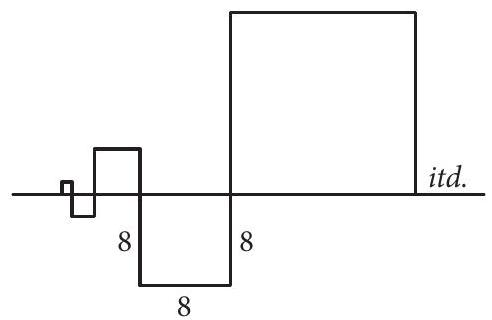
\includegraphics[max width=\textwidth, center]{2024_11_21_72158d4a4efa7dd894bcg-18}

Więcej arkuszy znajdziesz na stronie: \href{http://arkusze.pl}{arkusze.pl}\\

\includegraphics[max width=\textwidth, center]{2024_11_21_72158d4a4efa7dd894bcg-18(1)}

Odpowiedź:

Zadanie 31. (0-4)\\
W koszyku jest pięć kul o numerach 1, 2, 3, 6, 9. Losujemy kolejno bez zwracania trzy kule i zapisujemy ich numery, tworząc liczbę trzycyfrową: numer pierwszej wylosowanej kuli jest cyfrą setek, drugiej - cyfrą dziesiątek, a trzeciej - cyfrą jedności zapisanej liczby. Oblicz prawdopodobieństwo, że otrzymamy liczbę podzielną przez 3. Wynik podaj w postaci ułamka nieskracalnego.

\begin{center}
\begin{tabular}{|c|c|c|c|c|c|c|c|c|c|c|c|c|c|c|c|c|c|c|c|c|c|c|c|c|c|c|c|}
\hline
 &  &  &  &  &  &  &  &  &  &  &  &  &  &  &  &  &  &  &  &  &  &  &  &  &  &  &  \\
\hline
 &  &  &  &  &  &  &  &  &  &  &  &  &  &  &  &  &  &  &  &  &  &  &  &  &  &  &  \\
\hline
 &  &  &  &  &  &  &  &  &  &  &  &  &  &  &  &  &  &  &  &  &  &  &  &  &  &  &  \\
\hline
 &  &  &  &  &  &  &  &  &  &  &  &  &  &  &  &  &  &  &  &  &  &  &  &  &  &  &  \\
\hline
 &  &  &  &  &  &  &  &  &  &  &  &  &  &  &  &  &  &  &  &  &  &  &  &  &  &  &  \\
\hline
 &  &  &  &  &  &  &  &  &  &  &  &  &  &  &  &  &  &  &  &  &  &  &  &  &  &  &  \\
\hline
 &  &  &  &  &  &  &  &  &  &  &  &  &  &  &  &  &  &  &  &  &  &  &  &  &  &  &  \\
\hline
 &  &  &  &  &  &  &  &  &  &  &  &  &  &  &  &  &  &  &  &  &  &  &  &  &  &  &  \\
\hline
 &  &  &  &  &  &  &  &  &  &  &  &  &  &  &  &  &  &  &  &  &  &  &  &  &  &  &  \\
\hline
 &  &  &  &  &  &  &  &  &  &  &  &  &  &  &  &  &  &  &  &  &  &  &  &  &  &  &  \\
\hline
 &  &  &  &  &  &  &  &  &  &  &  &  &  &  &  &  &  &  &  &  &  &  &  &  &  &  &  \\
\hline
 &  &  &  &  &  &  &  &  &  &  &  &  &  &  &  &  &  &  &  &  &  &  &  &  &  &  &  \\
\hline
 &  &  &  &  &  &  &  &  &  &  &  &  &  &  &  &  &  &  &  &  &  &  &  &  &  &  &  \\
\hline
 &  &  &  &  &  &  &  &  &  &  &  &  &  &  &  &  &  &  &  &  &  &  &  &  &  &  &  \\
\hline
 &  &  &  &  &  &  &  &  &  &  &  &  &  &  &  &  &  &  &  &  &  &  &  &  &  &  &  \\
\hline
 &  &  &  &  &  &  &  &  &  &  &  &  &  &  &  &  &  &  &  &  &  &  &  &  &  &  &  \\
\hline
 &  &  &  &  &  &  &  &  &  &  &  &  &  &  &  &  &  &  &  &  &  &  &  &  &  &  &  \\
\hline
 &  &  &  &  &  &  &  &  &  &  &  &  &  &  &  &  &  &  &  &  &  &  &  &  &  &  &  \\
\hline
 &  &  &  &  &  &  &  &  &  &  &  &  &  &  &  &  &  &  &  &  &  &  &  &  &  &  &  \\
\hline
 &  &  &  &  &  &  &  &  &  &  &  &  &  &  &  &  &  &  &  &  &  &  &  &  &  &  &  \\
\hline
 &  &  &  &  &  &  &  &  &  &  &  &  &  &  &  &  &  &  &  &  &  &  &  &  &  &  &  \\
\hline
 &  &  &  &  &  &  &  &  &  &  &  &  &  &  &  &  &  &  &  &  &  &  &  &  &  &  &  \\
\hline
 &  &  &  &  &  &  &  &  &  &  &  &  &  &  &  &  &  &  &  &  &  &  &  &  &  &  &  \\
\hline
 &  &  &  &  &  &  &  &  &  &  &  &  &  &  &  &  &  &  &  &  &  &  &  &  &  &  &  \\
\hline
 &  &  &  &  &  &  &  &  &  &  &  &  &  &  &  &  &  &  &  &  &  &  &  &  &  &  &  \\
\hline
 &  &  &  &  &  &  &  &  &  &  &  &  &  &  &  &  &  &  &  &  &  &  &  &  &  &  &  \\
\hline
 &  &  &  &  &  &  &  &  &  &  &  &  &  &  &  &  &  &  &  &  &  &  &  &  &  &  &  \\
\hline
 &  &  &  &  &  &  &  &  &  &  &  &  &  &  &  &  &  &  &  &  &  &  &  &  &  &  &  \\
\hline
 &  &  &  &  &  &  &  &  &  &  &  &  &  &  &  &  &  &  &  &  &  &  &  &  &  &  &  \\
\hline
 &  &  &  &  &  &  &  &  &  &  &  &  &  &  &  &  &  &  &  &  &  &  &  &  &  &  &  \\
\hline
 &  &  &  &  &  &  &  &  &  &  &  &  &  &  &  &  &  &  &  &  &  &  &  &  &  &  &  \\
\hline
 &  &  &  &  &  &  &  &  &  &  &  &  &  &  &  &  &  &  &  &  &  &  &  &  &  &  &  \\
\hline
 &  &  &  &  &  &  &  &  &  &  &  &  &  &  &  &  &  &  &  &  &  &  &  &  &  &  &  \\
\hline
 &  &  &  &  &  &  &  &  &  &  &  &  &  &  &  &  &  &  &  &  &  &  &  &  &  &  &  \\
\hline
 &  &  &  &  &  &  &  &  &  &  &  &  &  &  &  &  &  &  &  &  &  &  &  &  &  &  &  \\
\hline
\end{tabular}
\end{center}

Odpowiedź:

\begin{center}
\begin{tabular}{|l|l|c|c|}
\hline
\multirow{2}{*}{\begin{tabular}{c}
Wypełnia \\
sprawdzający \\
\end{tabular}} & Nr zadania & 30 & 31 \\
\cline { 2 - 4 }
 & Maks. liczba pkt & 2 & 4 \\
\cline { 2 - 4 }
 & Uzyskana liczba pkt &  &  \\
\hline
\end{tabular}
\end{center}

Zadanie 32. (0-4)\\
W trójkącie prostokątnym \(A B C\) punkty \(A=(-4,1)\) i \(B=(7,-2)\) są końcami przeciwprostokątnej. Prosta o równaniu \(y=\frac{1}{3} x+\frac{7}{3}\) zawiera jedną z przyprostokątnych tego trójkąta. Oblicz długość środkowej \(B S\) w trójkącie \(A B C\).

Więcej arkuszy znajdziesz na stronie: \href{http://arkusze.pl}{arkusze.pl}\\

\includegraphics[max width=\textwidth, center]{2024_11_21_72158d4a4efa7dd894bcg-20}\\
Więcej arkuszy znajdziesz na stronie: \href{http://arkusze.pl}{arkusze.pl}\\

\includegraphics[max width=\textwidth, center]{2024_11_21_72158d4a4efa7dd894bcg-21}

Odpowiedź:

\begin{center}
\begin{tabular}{|l|l|c|}
\hline
\multirow{2}{*}{\begin{tabular}{c}
Wypełnia \\
sprawdzający \\
\end{tabular}} & Nr zadania & 32 \\
\cline { 2 - 3 }
 & Maks. liczba pkt & 4 \\
\cline { 2 - 3 }
 & Uzyskana liczba pkt &  \\
\hline
\end{tabular}
\end{center}

Zadanie 33. (0-5)\\
W graniastosłupie prawidłowym czworokątnym (zobacz rysunek poniżej) punkt \(O\) jest punktem przecięcia przekątnych podstawy dolnej, a odcinek \(O C^{\prime}\) jest o 4 dłuższy od przekątnej podstawy. Graniastosłup ten przecięto płaszczyzną przechodzącą przez przekątną \(B D\) podstawy dolnej i wierzchołek \(C^{\prime}\) podstawy górnej. Pole figury otrzymanej w wyniku przekroju jest równe 48. Zaznacz tę figurę na rysunku poniżej i oblicz objętość graniastosłupa.\\
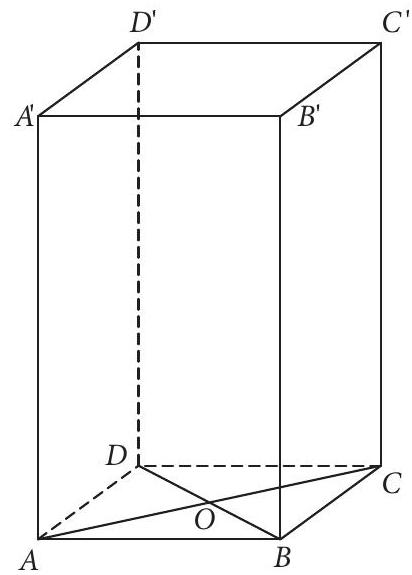
\includegraphics[max width=\textwidth, center]{2024_11_21_72158d4a4efa7dd894bcg-22}\\

\includegraphics[max width=\textwidth, center]{2024_11_21_72158d4a4efa7dd894bcg-22(1)}\\
Więcej arkuszy znajdziesz na stronie: \href{http://arkusze.pl}{arkusze.pl}\\

\includegraphics[max width=\textwidth, center]{2024_11_21_72158d4a4efa7dd894bcg-23}

Odpowiedź:

\begin{center}
\begin{tabular}{|l|l|c|}
\hline
\multirow{2}{*}{\begin{tabular}{c}
Wypełnia \\
sprawdzający \\
\end{tabular}} & Nr zadania & 33 \\
\cline { 2 - 3 }
 & Maks. liczba pkt & 5 \\
\cline { 2 - 3 }
 & Uzyskana liczba pkt &  \\
\hline
\end{tabular}
\end{center}

\begin{center}

\includegraphics[max width=\textwidth]{2024_11_21_72158d4a4efa7dd894bcg-24}
\end{center}

\section*{WPISUJE ZDAJĄCY}
\begin{center}
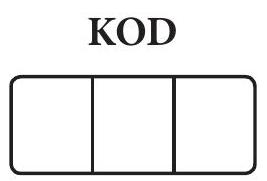
\includegraphics[max width=\textwidth]{2024_11_21_72158d4a4efa7dd894bcg-25}
\end{center}

IMIĘ I NAZWISKO *

\begin{itemize}
  \item nieobowiązkowe
\end{itemize}

KARTA ODPOWIEDZI

\begin{center}
\begin{tabular}{|c|c|c|c|c|c|}
\hline
 & Nr &  & Odpo & iedzi &  \\
\hline
 & 1 & A & B & C & D \\
\hline
 & 2 & A & B & C & D \\
\hline
 & 3 & A & B & C & D \\
\hline
 & 4 & A & B & C & D \\
\hline
D & 5 & A & B & C & D \\
\hline
民్ట & 6 & A & B & C & D \\
\hline
들 & 7 & A & B & C & C \\
\hline
\( \ddot{~} \) & 8 & A & B & C & D \\
\hline
응 & 9 & A & B & C & D \\
\hline
ঞ్a & 10 & A & B & C & D \\
\hline
位 & 11 & A & B & C & D \\
\hline
\( \stackrel{N}{\theta} \) & 12 & A & B & C & D \\
\hline
है & 13 & A & B & C & D \\
\hline
N્ & 14 & A & B & C & D \\
\hline
茜 & 15 & A & B & C & D \\
\hline

\includegraphics[max width=\textwidth]{2024_11_21_72158d4a4efa7dd894bcg-25(1)}
 & 16 & A & B & C & D \\
\hline
\( 3 \) & 17 & A & B & C & D \\
\hline
 & 18 & A & B & C & D \\
\hline
 & 19 & A & B & C & D \\
\hline
 & 20 & A & B & C & D \\
\hline
 & 21 & A & B & C & D \\
\hline
 & 22 & A & B & C & D \\
\hline
 & 23 & A & B & (C) & D \\
\hline
\end{tabular}
\end{center}

WYPEENIA SPRAWDZAJĄCY

\begin{center}
\begin{tabular}{|c|c|c|c|c|c|c|}
\hline
\multirow{2}{*}{\begin{tabular}{c}
Nr \\
zad. \\
\end{tabular}} & \multicolumn{6}{|c|}{Punkty} \\
\hline
 & \(\mathbf{0}\) & \(\mathbf{1}\) & \(\mathbf{2}\) & \(\mathbf{3}\) & \(\mathbf{4}\) & \(\mathbf{5}\) \\
\hline
\(\mathbf{2 4}\) & \(\square\) & \(\square\) & \(\square\) &  &  &  \\
\hline
\(\mathbf{2 5}\) & \(\square\) & \(\square\) & \(\square\) &  &  &  \\
\hline
\(\mathbf{2 6}\) & \(\square\) & \(\square\) & \(\square\) &  &  &  \\
\hline
\(\mathbf{2 7}\) & \(\square\) & \(\square\) & \(\square\) &  &  &  \\
\hline
\(\mathbf{2 8}\) & \(\square\) & \(\square\) & \(\square\) &  &  &  \\
\hline
\(\mathbf{2 9}\) & \(\square\) & \(\square\) & \(\square\) &  &  &  \\
\hline
\(\mathbf{3 0}\) & \(\square\) & \(\square\) & \(\square\) &  &  &  \\
\hline
\(\mathbf{3 1}\) & \(\square\) & \(\square\) & \(\square\) & \(\square\) & \(\square\) &  \\
\hline
\(\mathbf{3 2}\) & \(\square\) & \(\square\) & \(\square\) & \(\square\) & \(\square\) &  \\
\hline
\(\mathbf{3 3}\) & \(\square\) & \(\square\) & \(\square\) & \(\square\) & \(\square\) & \(\square\) \\
\hline
\end{tabular}
\end{center}


\end{document}